\chapter{ChapterName}
\label{chap1}

\section{Section}

We can insert and reference figures and stuff, look at the figure \ref{fig:fa}-A.

% insert figure
\begin{figure}[ht]
\centering
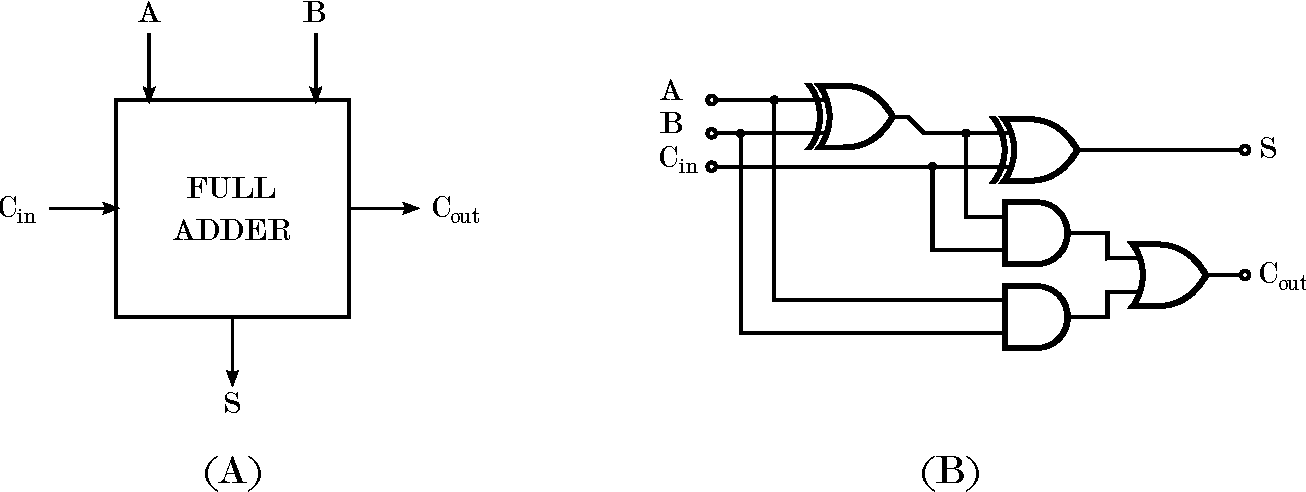
\includegraphics[width=\textwidth]{chapters/figures/fa} 
\caption{This is a caption for the figure}
\label{fig:fa}
\end{figure}

We can also make and reference tables, look at the table \ref{tab:1}.

% create table
\begin{table}[ht]
\centering
\begin{tabular}{ccc}
\toprule
A B Cin & S & Cout\\
\midrule
0 0 0 & 0 & 0\\
1 0 0 & 1 & 0\\
0 1 0 & 1 & 0\\
1 1 0 & 0 & 1\\
0 0 1 & 1 & 0\\
1 0 1 & 0 & 1\\
0 1 1 & 0 & 1\\
1 1 1 & 1 & 1\\
\bottomrule
\end{tabular}
\caption{Truth table of a 1-bit full adder.}
\label{tab:1}
\end{table}
	
We can also write equations and stuff, like equations \ref{eq:1} and \ref{eq:2}

\begin{equation}
S = A \oplus B \oplus C_{in}
\label{eq:1}
\end{equation}

\begin{equation}
C_{out} = AB + C_{in}( A \oplus B)
\label{eq:2}
\end{equation}
	
\subsection{SubSection}

We can read data from a file with verbatiminput:

\verbatiminput{chapters/files/planar_FA_area_power.txt}  

% You can also include some text in this way:
%	\begin{verbatim}
%		text here
%	\end{verbatim}

% Below is shown how to create an itemize. An alternative to itemize is enumerate that allows you to generate a numbered list. It is used in the same way as itemize:
%	\begin{enumerate}
%		\item bla1
%		\item bla2
%		\item bla3
%	\end{enumerate}

Beryyy info:
\begin{itemize}
\item Delay = 3 clock cycles;
\item Area = $2.7\ \mu m^2$;
\item Power = $10.53\ \mu W$.
\end{itemize}
	
\section{Another Section}

This is another section with stuff.\\
\dots \dots \dots \\
\dots \dots \\
\dots